\section{Modelo Proposto}
\label{cap:modelo proposto}


O protótipo AppMan é uma implementação simplificada do GRAND. Ele usa a ferramenta JavaCC para implementar o {\it parsing} e interpretação da GRID-ADL. A Figura 2 representa um possível cenário do AppMan sendo executado sobre um ambiente de grade.

O passo 1 da figura representa o usuário submetendo um arquivo de descrição na linguagem GRID-ADL. Esse arquivo é analisado e o grafo de aplicação é feito na memória. Um algoritmo é executado e os sub-DAGs do grafo de aplicação é obtido. O {\it Application Manager} (AM) é inicializado. Então o AM instância {\it Submission Managers} (SM) no passo 2 e distribui alguns subgrafos para os SMs. Os arquivos de entrada e os executáveis são obtidos através de um {\it web server} (passo 3). Na sua atual implementação, AppMan necessita que o usuário indique as máquinas onde os SMs irão ser executados. Com essa simplificação um novo SM é instanciado para cada aplicação em cada máquina especificada. Após a criação dos SMs, o AM determina sub-grafos para cada SM. Os SMs informam para o AM o progresso das tarefas. Cada SM, independentemente, verifica a lista das máquinas disponíveis e escolhe aleatoriamente um nó para executar a tarefa. Antes de iniciar a execução de uma tarefa, o AppMan transfere todos arquivos de entradas especificados na descrição GRID-ADL para um diretório temporário no nó remoto onde a tarefa será executada. O arquivo de transferência é executado automaticamente. Então, cada SM recupera a informação atualizada através do serviço de informação do EXEHDA sobre os nós avaliados. Cada SM escolhe onde irá executar estas tarefas aleatoriamente. Imediatamente um {\it Task Manameger} (TM) é instanciado criando a tarefa remota e monitorando até que a execução da tarefa termine (passo 4).

\begin{figure}[hbtp]
\center
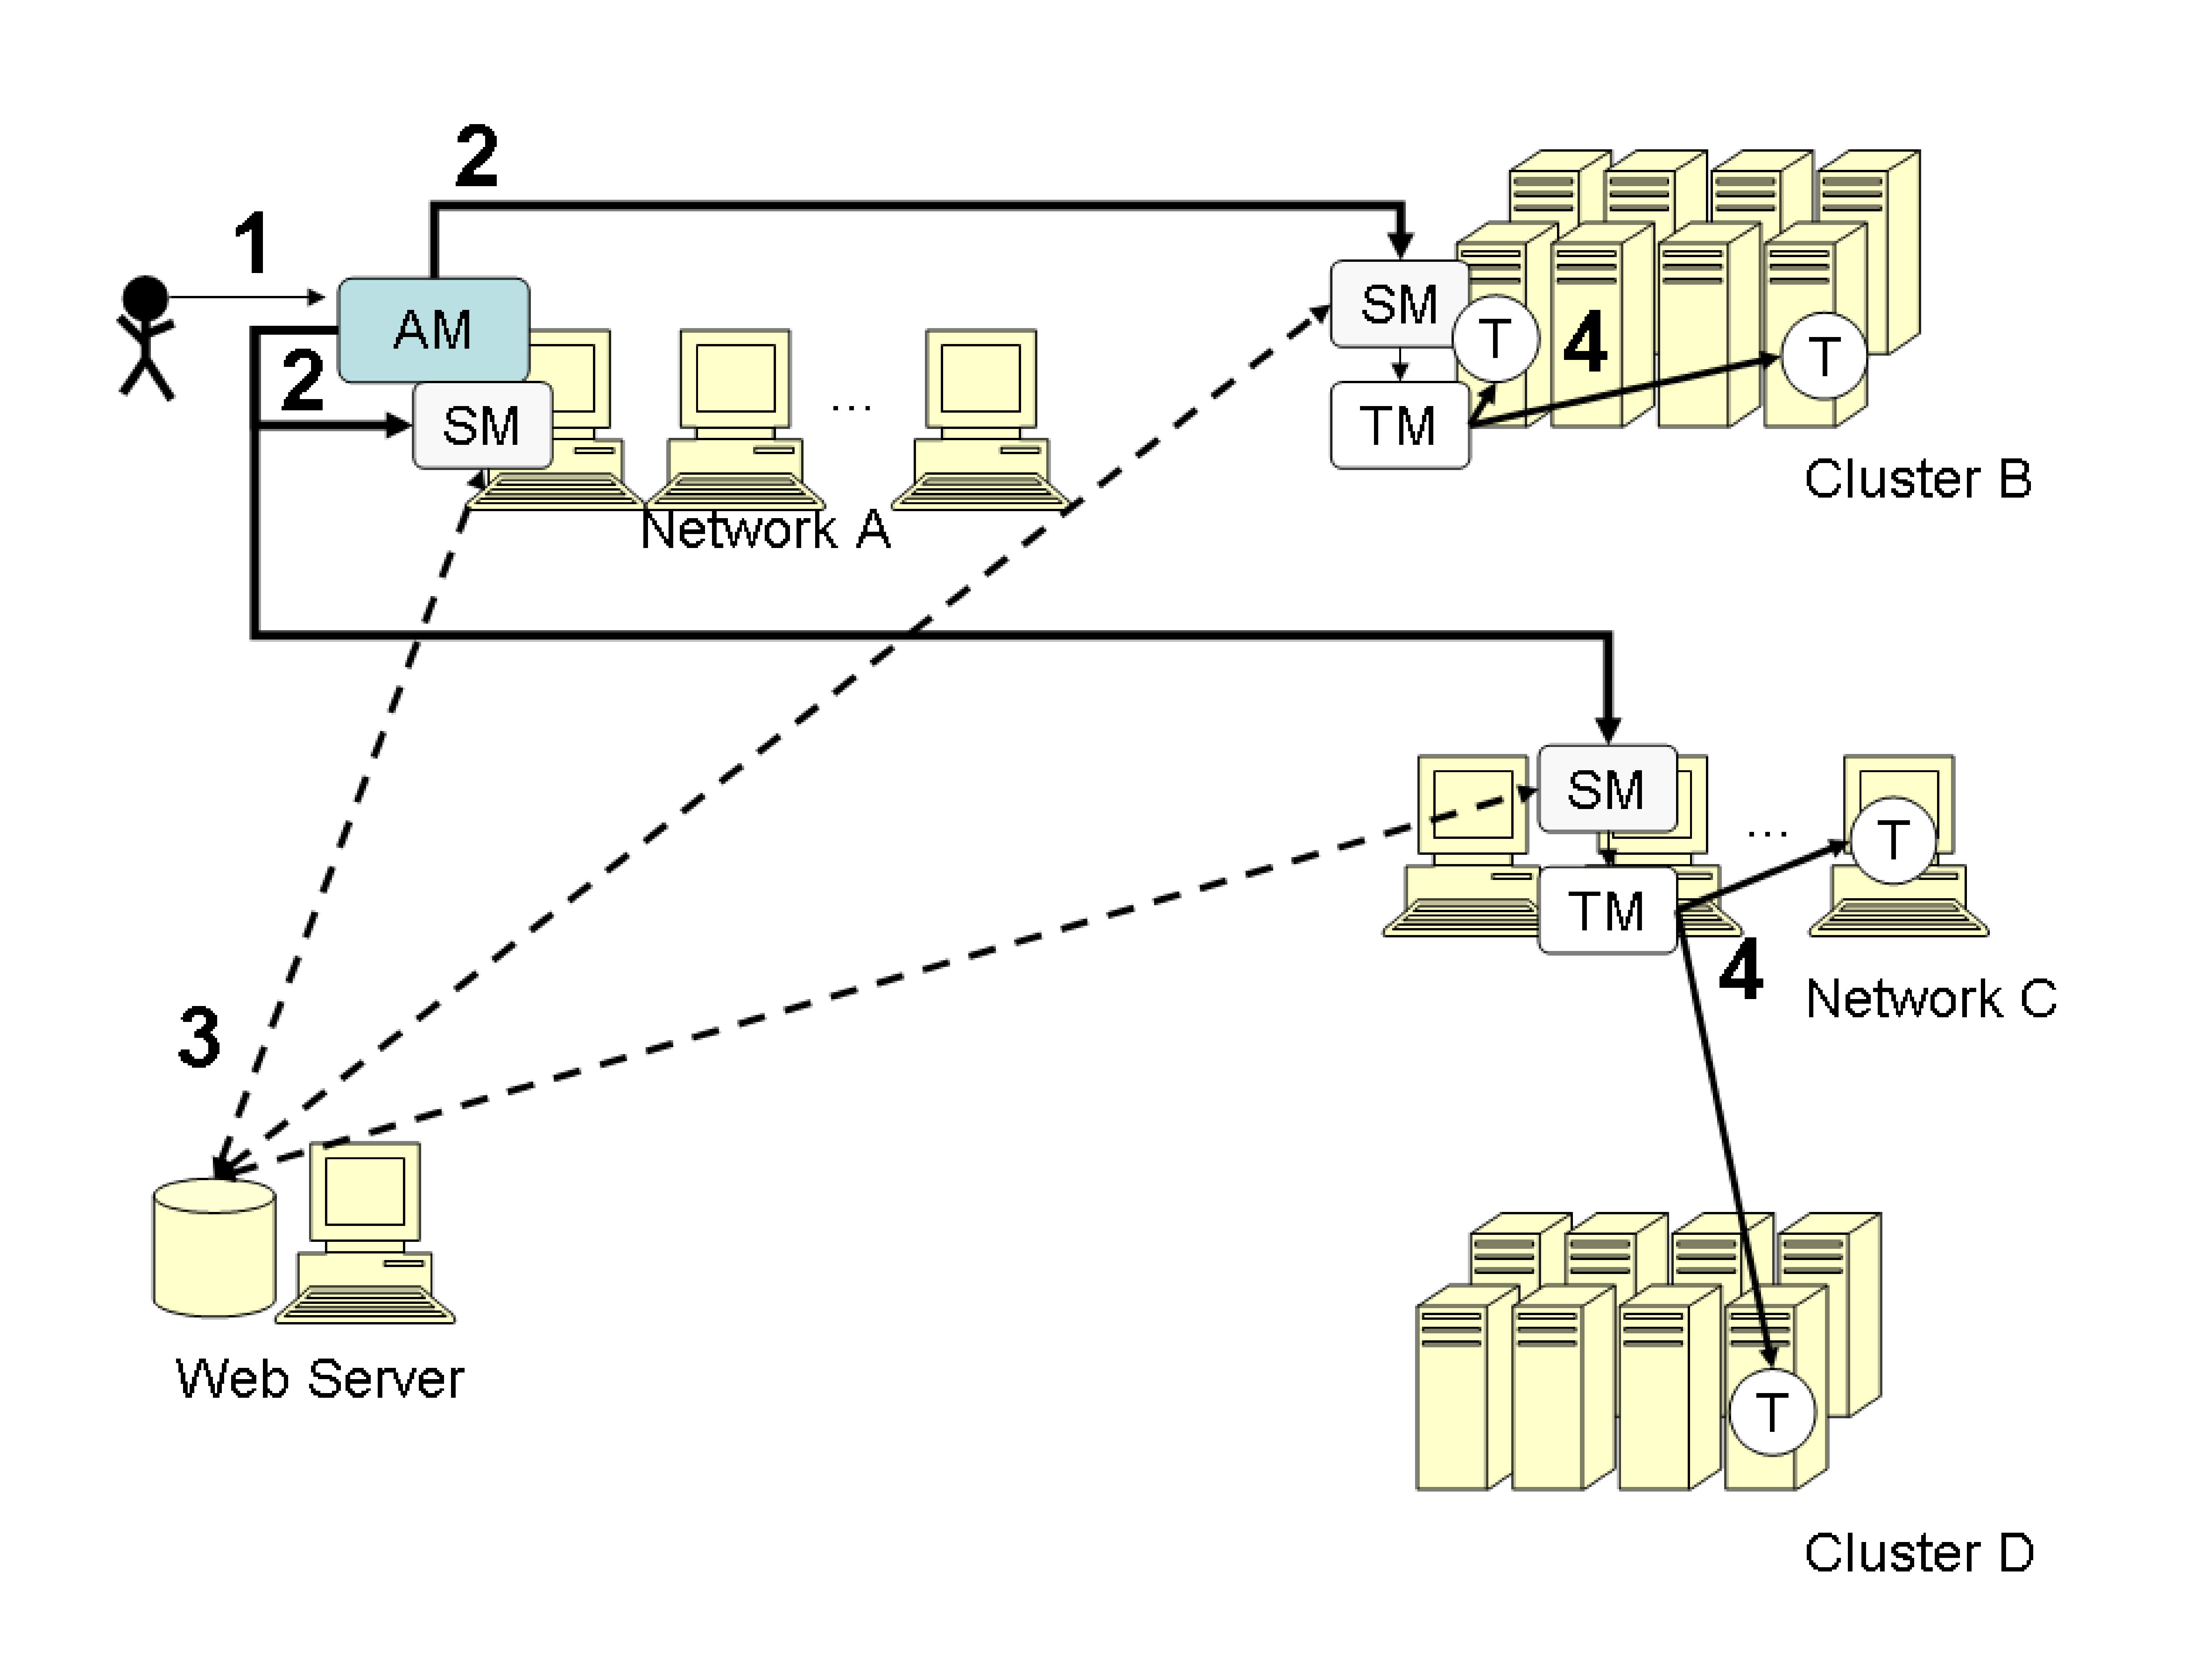
\includegraphics[scale=.1]{img/AppMan.eps}
\label{AppMan}
\caption{AppMan executando principais passos}
\end{figure}

Como sugere o modelo GRAND, o AppMan não possibilita o escalonamento através de outros RMSs. É necessário que o EXEHDA e o AppMan estejam presentes em todos nós da grade. Integrar o AppMan com outros RMS possibilitará uma maior escalabilidade da grade e também possibilitará uma aproximação do AppMan ao que sugere o modelo GRAND. Os nós principais de cada {\it cluster} que compõem a base possuem nós abaixo delas. O AppMan espera um serviço de compartilhamento de arquivo entre os nós e base. Isto é, mais uma característica que impossibilita o uso de nós da grade sem NFS, como existente na parceria LNCC/Petrópolis-RJ, pelo AppMan.

Uma especificação {\it Distributed Resource Management Application} \cite{Rajic2002} desenvolvida pelo OGF, tem por objetivo abstrair as diferenças dos RMS e fornecer uma API visando facilitar a integração de aplicações. O escopo da DRMAA é limitada a submissão, monitoramento e controle das tarefas além de retornar status de conclusão de uma tarefa. Inicialmente implementada na linguagem C, atualmente possui uma implementação na linguagem Java, apesar de oferecer suporte apenas para o {\it Sun Grid Engine} \cite{Templeton}.

Vários relatórios técnicos N1™ Grid Engine \cite{Templeton2006}, GridWay \cite{Herrera2007}, Condor \cite{Troeger2007} e PBS \cite{Ciesnik2007} existentes da implementação DRMAA, concluem positivamente. Além disso demonstraram uma pequena necessidade de inteferência no código dos RMSs citados.

Em um primeiro estudo da documentação do AppMan pode-se notar duas principais classes, {\it TaskManager} (Figura 3) e {\it SubmissionManager}. A classe {\it SubmissionManager} implementa os métodos da {\it Interface SubmissionManagerRemote} a qual possui os métodos que recuperam informações das tarefas executadas remotamente e o metódo da geração do grafo da aplicação. A classe {\it TaskManager } implementa a interface {\it TaskManagerRemote} contendo os métodos tais como os que adicionam tarefas na lista de execução remota.

\begin{figure}[h]
\center
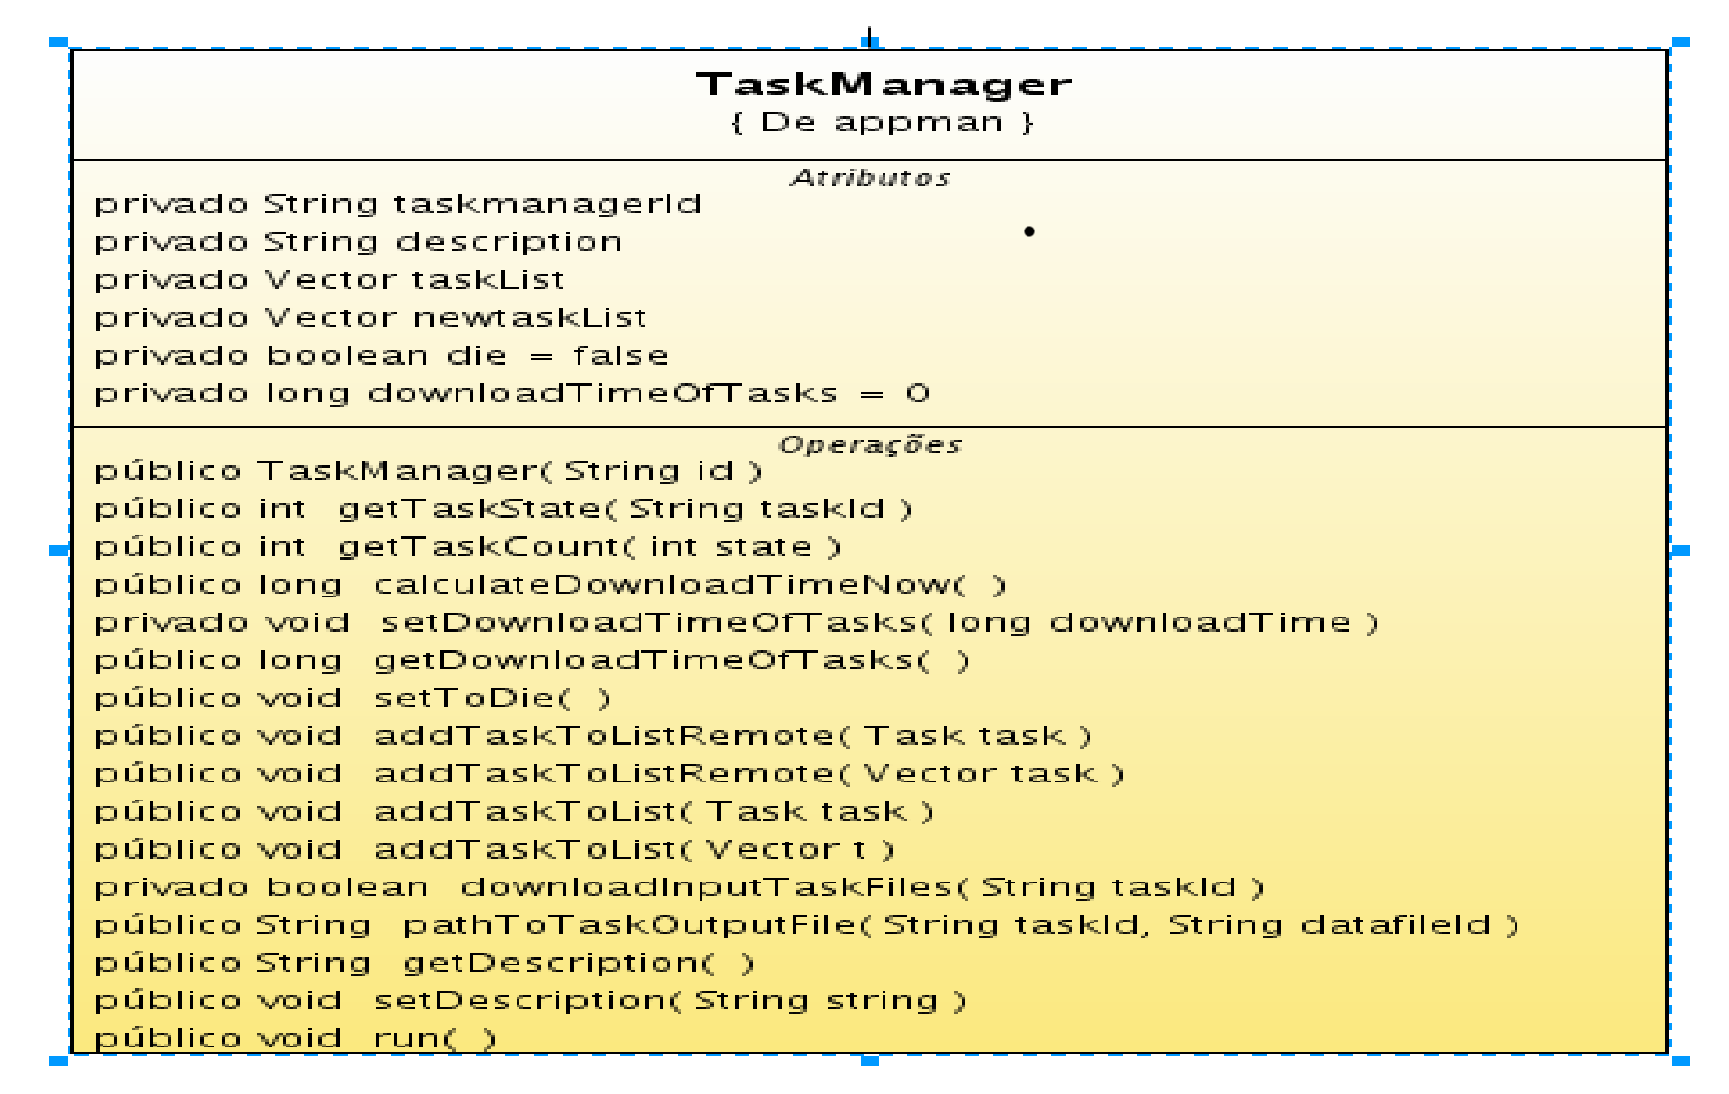
\includegraphics[scale=.4]{img/TaskManager.eps}
\label{TaskManager}
\caption{Classe TaskManager}
\end{figure}

Baseado no que foi analisado até o momento da confecção deste artigo, notou-se a necessidade de alteração na {\it Interface TaskManagerRemote} onde necessitará ser adicionado métodos que implementarão as especificações da DRMAA. Essa seria a melhor forma de implementação com a mínima interferência no código atual. Principalmente por existirem trabalhos nessa área \cite{Nobres2007}.

A presente proposta de pesquisa proporcionará uma maior dispersão geográfica para o AppMan pois, novos domínios adimistrativos (instituições) poderão fazer parte da grade em que se encontra. Contribuiria, também, para o AppMan ficar próximo de atingir o que propõem o modelo GRAND resolvendo o problema da necessidade do EXEHDA/AppMan estarem presentes em todos nós da grade. 

A Figura 4 demonstra como deverá ficar o funcionamento do AppMan após a realização do trabalho proposto. Os TMs nos nós locais contatam RMSs remotos despachando as tarefas para esses RMSs.

\begin{figure}[hpts]
\center
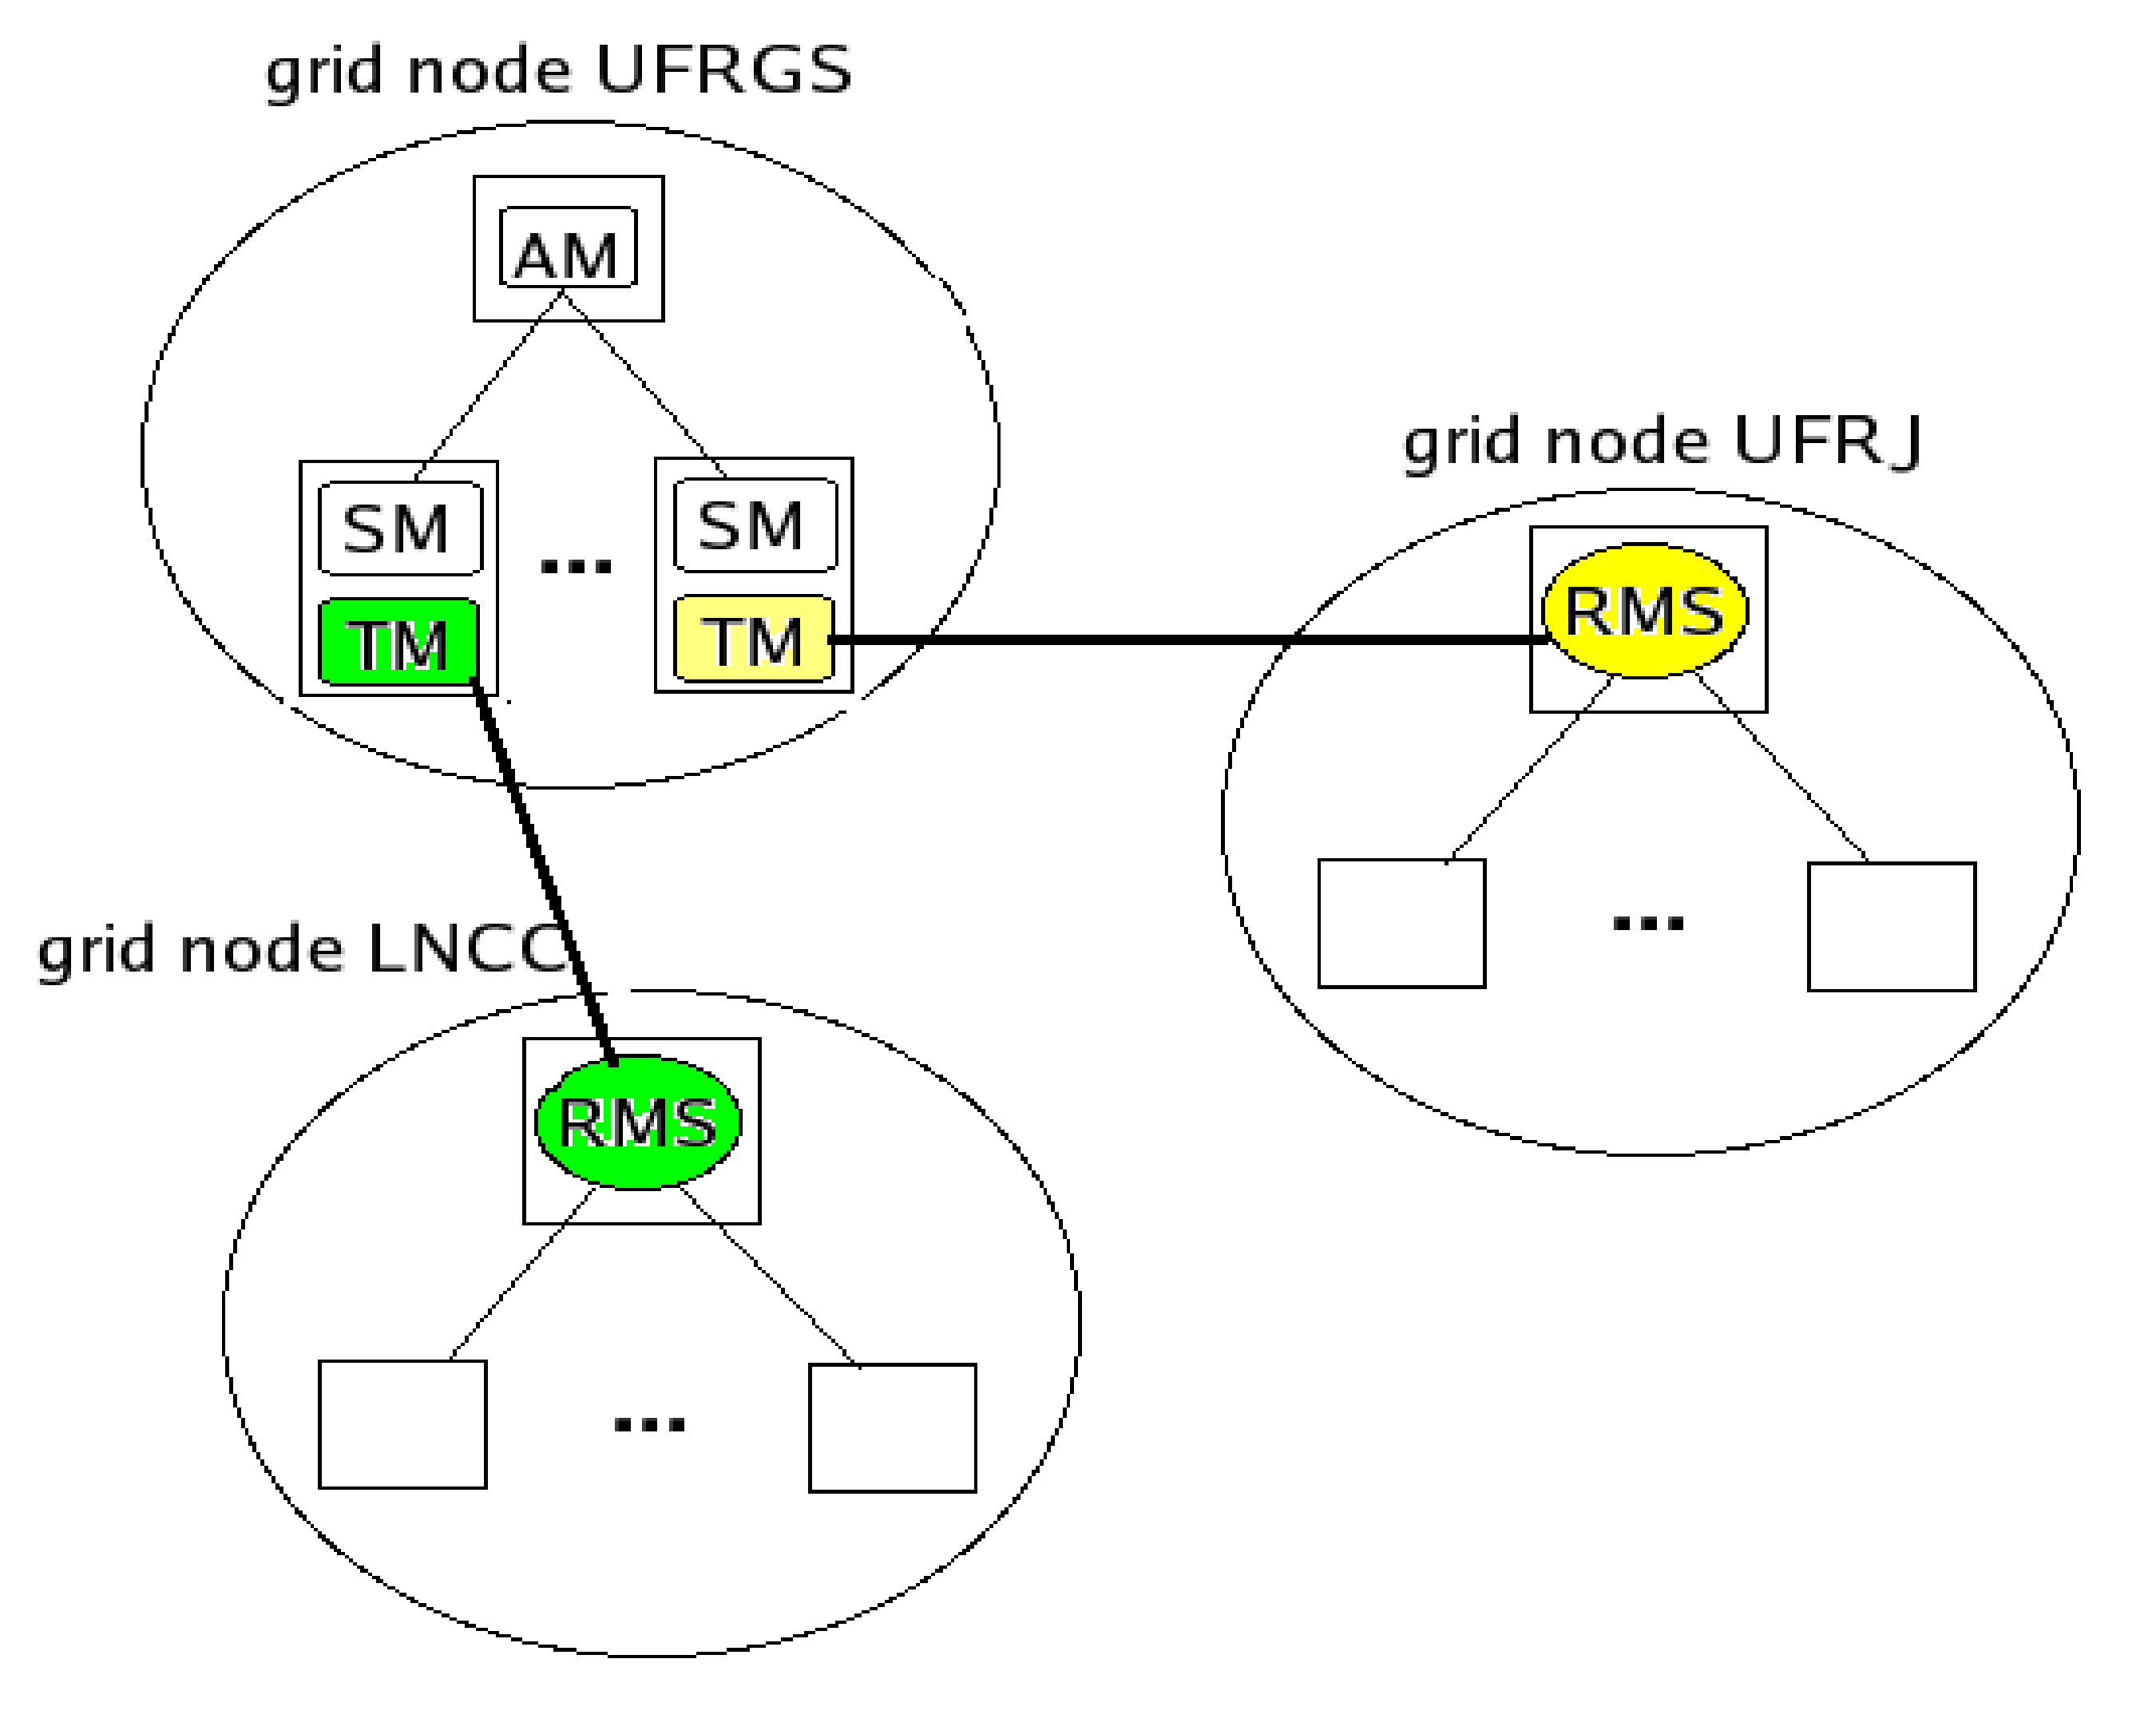
\includegraphics[scale=.2]{img/AppManRMS.eps}
\label{AppManRMS}
\caption{AppMan executando em um cenário com TMs comunicando com RMS}
\end{figure}

O modelo proposto para o TCC consiste em avaliar se a especificação DRMAA atende as necessidades do AppMan bem como realizar a integração do AppMan ao menos com um RMS.
